\subsection{Detection Pipelines}

Transit surveys must distinguish genuine planetary transits from signals affected by stellar variability, instrumental systematics, and astrophysical false positives. Detection pipelines are therefore used to calibrate the raw photometry, remove long-timescale trends, search for periodic transit-like signals, and identify candidates requiring further classification.

Before transit-like signals can be searched or classified, photometric light curves must be corrected for instrumental systematics and long-timescale stellar variability. For \textit{Kepler}, this processing produced calibrated and detrended light-curve products that are better suited for identifying short-duration transit events \citep{Jenkins_TCE_Label, 2018ApJS..235...38T}. This preprocessing context is important because the machine-learning models in this work are applied to processed light curves rather than raw detector measurements.

After preprocessing, transit-search algorithms are used to identify periodic decreases in stellar flux. Methods such as Box Least Squares (BLS) search for repeating, box-shaped dips that are consistent with transit-like events \citep{BLS_Algorithm}. In the \textit{Kepler} pipeline, the Transiting Planet Search (TPS) algorithm performed a similar role by searching for periodic transit-like signals in the processed light curves \citep{Jenkins_TCE_Label}.

Signals exceeding the detection threshold are labelled as Threshold Crossing Events (TCEs). However, a TCE does not necessarily correspond to a planet, since eclipsing binaries, stellar variability, and instrumental effects can also produce transit-like signals. The identification of TCEs therefore marks the transition from signal detection to candidate classification, where the goal is to separate genuine planetary transits from false positives.

\subsubsection{Neural Networks for Transit Classification} 

Machine learning methods are useful for transit classification because they can learn patterns from labelled light curves and apply them consistently across large datasets \citep{2018AJ....155..147Z}. In supervised classification, the model is trained on examples with known labels, allowing it to adjust its internal parameters to reduce prediction errors. Once trained, the model is evaluated on separate test data to assess how well it generalizes to unseen light curves.

The \textit{Kepler} archive provides a useful source of labelled examples, including confirmed planetary transits, eclipsing binaries, and other false-positive signals that can be used to develop automated classification methods \citep{2018ApJS..235...38T}. Many machine-learning studies further process these light curves by phase-folding them over the detected orbital period, producing a single combined transit profile that makes the transit shape easier to classify \citep{2018AJ....155...94S}. In contrast, this work uses fixed-length light-curve segments, allowing the models to classify transit-like signals without first reducing each target to a phase-folded profile.

Convolutional neural networks (CNNs) are well suited to time-series data such as stellar light curves because they can identify local patterns within the signal, including the depth, duration, and shape of transit-like events. This allows CNNs to distinguish planetary transits from common false positives such as eclipsing binaries or stellar variability without requiring every feature to be manually defined. A notable example is \citet{2018AJ....155...94S}, who developed the Astronet CNN model and applied it to \textit{Kepler} light curves, identifying several previously missed exoplanet candidates.

\begin{comment}
\textit{Kepler} data contains continuous variability that are not caused by the planet but by the stars and instrument limitations. To manage this, before conducting research and parameter estimation, a preprocessing step is required \citep{2018ApJS..235...38T}.  

The most well-known and well-developed pipeline comes from the \textit{Kepler} mission. Their Science Processing Pipeline consists of several modules with the focus of slowly calibrating and filtering the raw collected data \citep{Jenkins_TCE_Label}. The order of processes is:

\begin{enumerate}
    \item Calibration (CAL) - Corrects detector level artifacts with focus on bias, gain variations, and electronic noise
    \item Photometric Analysis (PA) - Conducts aperture photometry for each star at each cadence by summing flux within a predefined set of CCD pixels
\end{enumerate}

Following this, the \textit{Kepler} mission focuses on managing error and trends caused by spacecraft motion and temperature changes in the instrumentation. This is called Presearch Data Conditioning (PDC) and it works by fitting co-trending basis vectors to remove typical trends.

From here, astronomers can take different approaches in handling the \textit{Kepler} processed data. The first aspect to focus on is typically brightness fluctuations caused by factors such as rotation, star spots, and magnetic activity. With planetary transits usually occurring over a few hours, these variations occur on much larger timescales \citep{2012IAUS..285..364M}. A simple high pass filter then helps to remove the low-frequency variability in a time series dataset. This process works to preserve the shorter duration transit signals in exoplanet detection. Furthermore, polynomial detrending, median filters, and spline fitting are also commonly used approaches \citep{2006MNRAS.373..231P, 2011ApJS..197....6G}.

The next step is to normalize and stitch the various quadrants together. This gives a continuous light curve which can now be used for transit detection. This cleaning stage is critical because the transit signals targeted by surveys such as \textit{Kepler} are often extremely small. For example, the transit depth produced by an Earth-sized planet orbiting a Sun-like star is approximately 80 parts per million, requiring extremely precise noise removal to reliably detect \citep{2011ApJS..197....6G}. Although the overall philosophy of preprocessing is similar across missions, different surveys implement their filtering procedures with small variations. 

For TESS, similar preprocessing is provided through mission pipeline products such as SAP and PDCSAP light curves, where instrumental trends are reduced prior to transit searches \citep{TCE_Labelling}. In addition, the Quick-Look Pipeline (QLP) produces detrended light curves for many full-frame image targets \citep{2020RNAAS...4..204H}. Although the implementation differs from \textit{Kepler}, the overall goal remains the same: to suppress instrumental errors and long-timescale variability while preserving short-duration transit signals. More generally, both missions rely on preprocessing to reduce instrumental and stellar noise so that periodic transit signals can be detected with sufficient signal-to-noise ratio.

\subsection{Algorithms}

With the raw data detrended and processed, the next step is looking for potential transits within the time series. As there are a high number of light curves to search through, the process is primarily automated. By looking for the short dips and periodic repetition, researchers try to identify box shaped changes in the dataset.

This introduces the most common search method known as the Box-Least Squares (BLS) algorithm. Originally developed by \cite{BLS_Algorithm}, BLS is a process which attempts to fit a box shape over the flux dip. Although it is less useful for parameter estimation, at this stage astronomers are primarily concerned with identifying candidate exoplanet signals rather than proof of an exoplanet. A signal-to-noise ratio is then calculated from this fit and used as a detection statistic for the candidate exoplanet. Appendix \ref{sec:Transit_Detection_Statistic} shows the calculation of this significance value. \cite{2019A&A...623A..39H} take the BLS method further and create the Transit Least Squares (TLS) method. It adds limb darkening into the fitting which improves detection and limits false confirmations. Figure~\ref{fig:BLS&TLS} provides a simple comparison of the BLS and TLS methods in terms of fitting and residuals.

\begin{figure}[h]
    \centering
    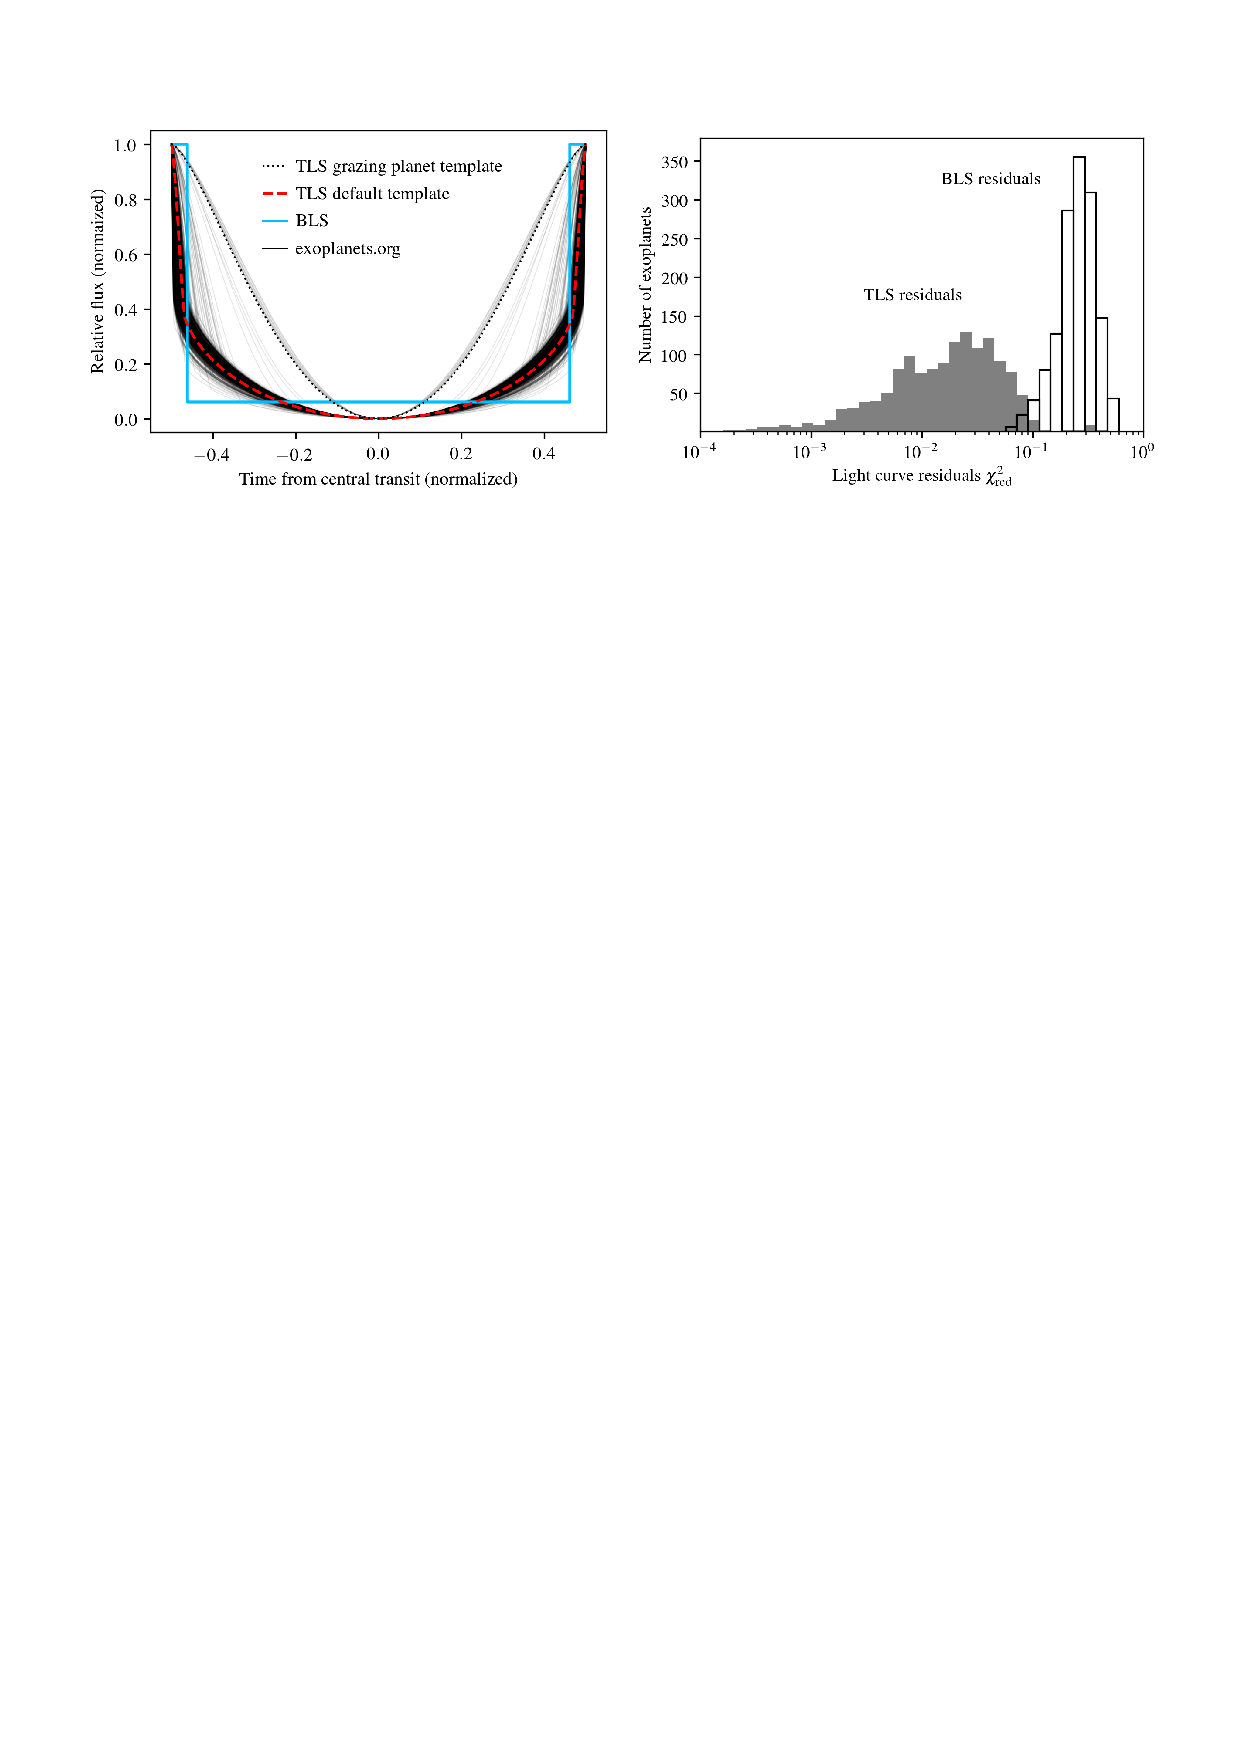
\includegraphics[width=1.0\linewidth]{paper/figures/other_papers/BLS&TLS.pdf}
    \caption{\citet{2019A&A...623A..39H} compare the BLS and TLS methods. The blue line represents the simple box-shaped model used to identify transit-like signals. TLS provides a more realistic representation of the transit shape, and the histogram illustrates the improvement in fit achieved relative to BLS. \cite{2019A&A...623A..39H} (Figure 2).}
    \label{fig:BLS&TLS}
\end{figure}

The \textit{Kepler} mission conducts a specialized process called the Transiting Planet Search (TPS) algorithm \citep{Jenkins_TCE_Label}. It employs a wavelet based matched filter which looks for periodic transit-like signals with durations ranging from 1 to 16 hours. If a potential detection returns a transit detection statistic greater than 7.1$\sigma$, it is labelled as a Threshold Crossing Event (TCE). A TCE does not necessarily imply the presence of a planet. Many of these signals can come from the mentioned challenges in Section~\ref{sec:Detection_Challenges}. Consequently, additional vetting stages are required to determine whether a TCE corresponds to a genuine exoplanet candidate.

The identification of TCEs is a major step in the detection pipeline. Moving forward from here, researchers finish signal detection and continue onto signal classification. The goal now is to distinguish true planetary transits from the wide variety of possible astrophysical and instrumental false positives.

\end{comment}